\section{Appendix}



\subsection{Computational Efficiency}
\label{subsec:throughput}

To evaluate the computational efficiency of our data generation pipeline, we measured the throughput using a model system consisting of an uncapped tetra-alanine peptide (AAAA). 
The fully solvated system comprised 1,682 atoms in total (of which 43 atoms were from the solute) surrounded by explicit water molecules with a 1.2~nm padding. 
All benchmarking runs were executed on a single NVIDIA A100 GPU.

We benchmarked two parallelization strategies and compared their throughput as a function of the number of concurrently running systems (Figure~\ref{fig:throughput_combined}).

The first strategy consists of conventional independent simulations at a constant temperature of 300~K. To maximize GPU utilization, we simulated multiple independent copies of the system concurrently, dispatching each run in isolation via its own dedicated system process.

The second strategy employs \gls{remd} \cite{qi2018replica}, which runs simulations at multiple temperatures and periodically exchanges configurations between replicas to improve conformational sampling. This approach helps avoid biased datasets that overrepresent only a limited set of conformations. For the \gls{remd} protocol, we leveraged the \texttt{reform} package \cite{chen_noe_reform} to orchestrate replica swaps. By default, the multi-threaded interface of \texttt{reform} does not support periodic boundary conditions. However, modeling the explicit solvent requires periodic boundary conditions to avoid surface artifacts. To overcome this limitation, we constructed a custom wrapper around \texttt{reform}'s single-threaded API, managing a dedicated thread per replica to parallelize execution while retaining support for periodic boundary conditions.


\begin{figure}[htbp]
    \centering
    % TODO: replace with combined throughput figure
    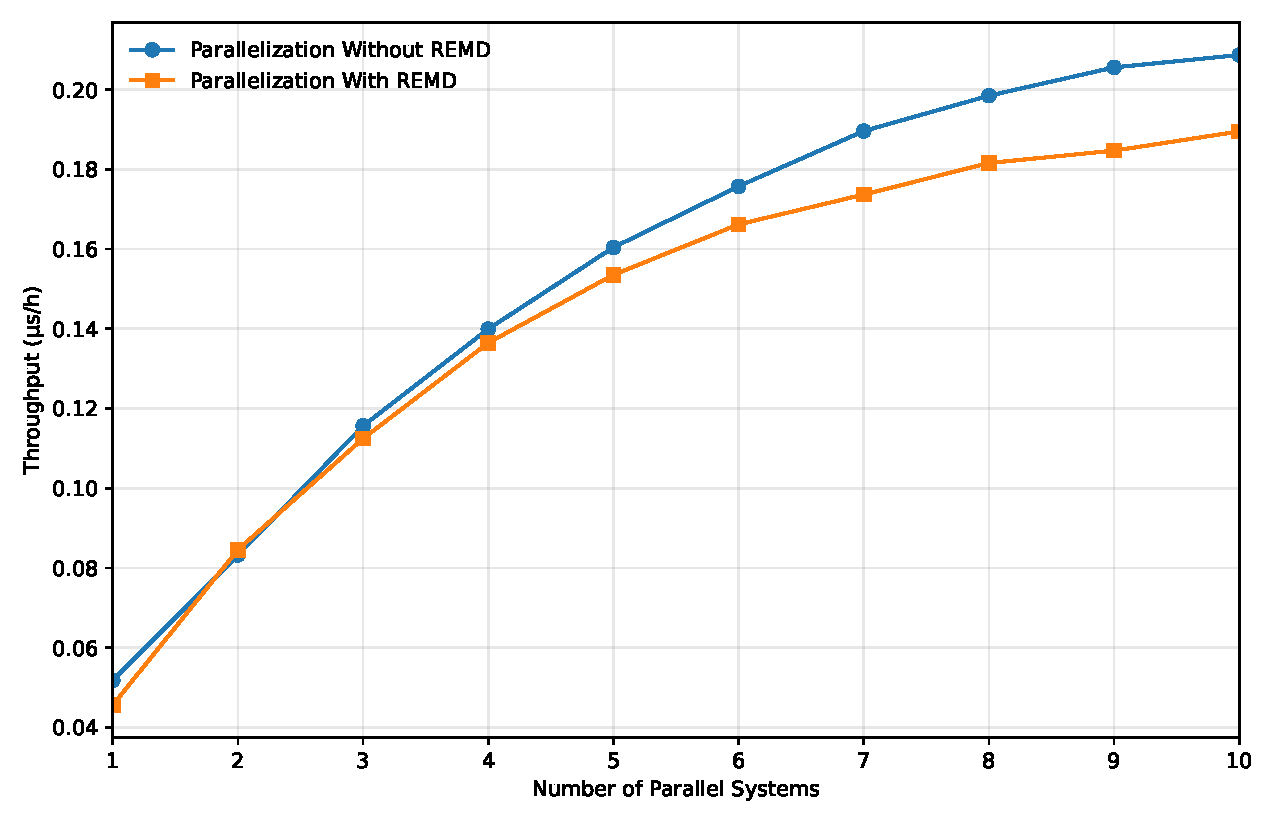
\includegraphics[width=0.7\linewidth]{images/throughput_AA_vs_solvated_upto10.pdf}
    \caption{Aggregate simulation throughput on a single NVIDIA A100 GPU as a function of the number of parallel systems, comparing independent parallelization at 300~K and the custom-parallelized \gls{remd} setup using the \texttt{reform} package. Both strategies are evaluated on the uncapped AAAA tetrapeptide system.}
    \label{fig:throughput_combined}
\end{figure}

In the end, we did not use \gls{remd} for the final data generation, as the computational overhead of running multiple replicas does not justify the improved sampling.


\subsection{Solvent Scaling with Sequence Length}

Because a fixed margin of water must surround the peptide in all three dimensions to avoid boundary artifacts, the total volume and therefore the number of solvent atoms scales cubically ($\mathcal{O}(L^3)$) with the sequence length $L$. This rapid addition of solvent atoms makes large-scale simulations of long peptides slow (Figure \ref{fig:system_scaling}).

\begin{figure}[htbp]
    \centering
    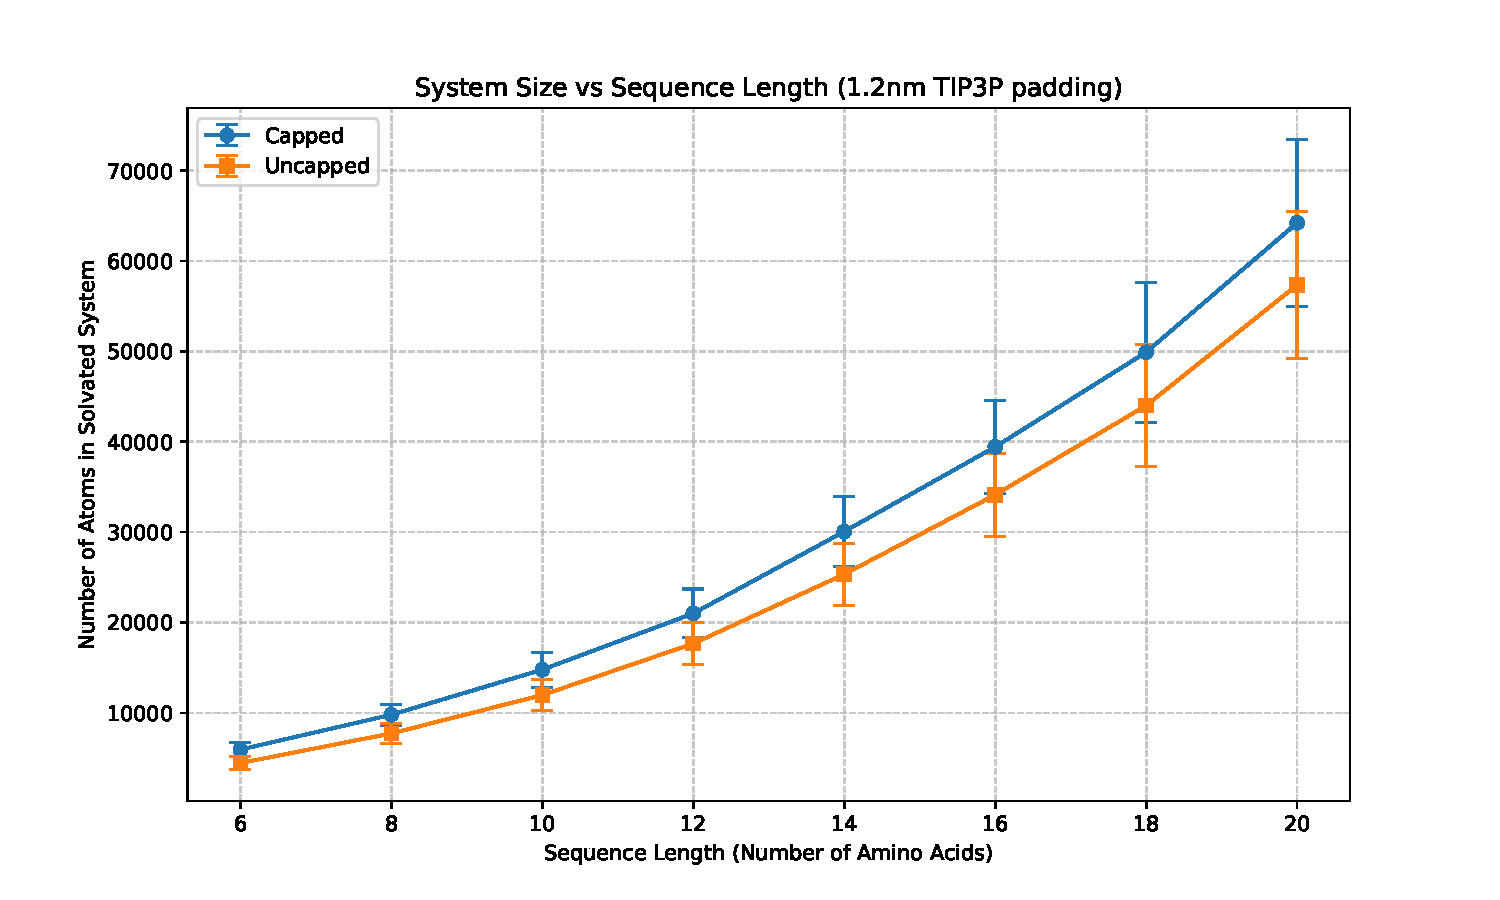
\includegraphics[width=0.7\linewidth]{images/scaling_plot.pdf}
    \caption{Number of explicitly solvated atoms (TIP3P with 1.2\,nm padding) plotted against sequence length for random combinations of 20 standard amino acids. A nonlinear increase in system size naturally emerges to encapsulate the expanding spatial volume of longer chains.}
    \label{fig:system_scaling}
\end{figure}


\subsection{Dataset Distributions}

To resolve both the thermodynamic conformational preferences and the underlying kinetic dynamics of the dipeptides and tetrapeptides, we perform a analysis comprising Ramachandran free energy surfaces and \gls{tica} \citep{perez2013identification}. 

Figure \ref{fig:dipeptide_kinetics_thermo} illustrates this relationship for four selected dipeptides (AF, HT, KL, QW). The upper panels display the Potential of Mean Force (PMF) projected onto the classical Ramachandran space ($\phi$, $\psi$), revealing the accessible thermodynamic states and free energy minima. The lower panels show the corresponding \gls{tica} projections of the kinetically separated components (TIC 0 and TIC 1), showing the slowest structural transitions between these metastable minima.
Figure \ref{fig:tetrapeptide_kinetics_thermo} extends this analysis to four tetrapeptides (AGPW, CNLV, DERS, FITL).

\begin{figure*}[htbp]
    \centering
    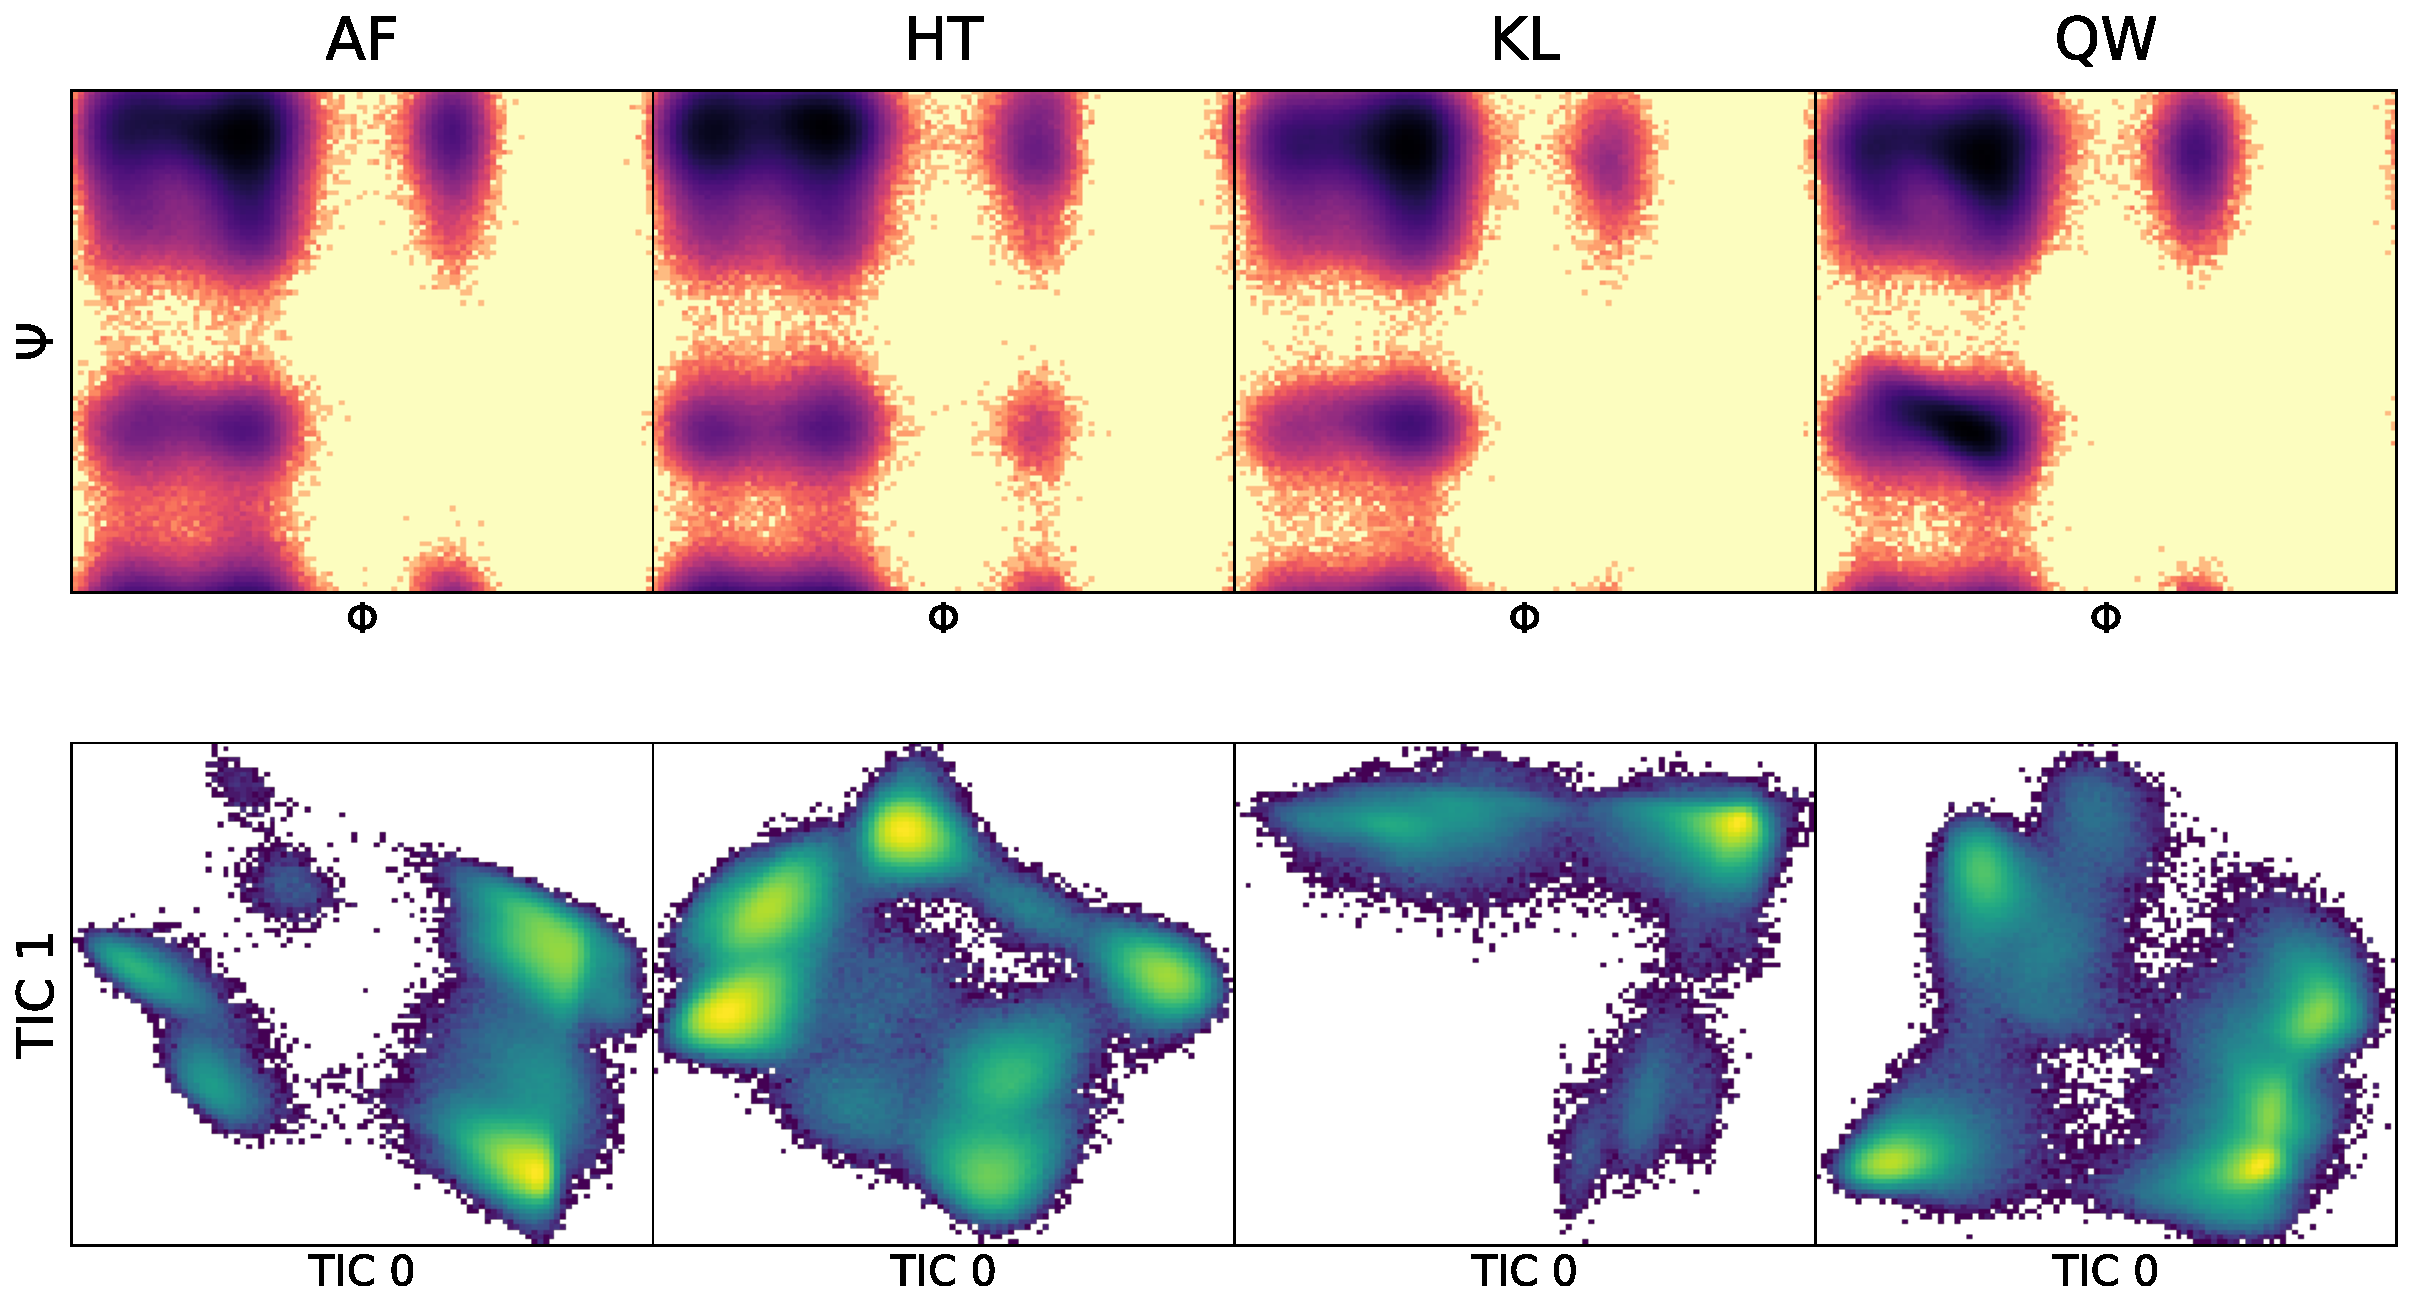
\includegraphics[width=\linewidth]{images/custom_grid_FA_HT_KL_QW.pdf}
    \caption{Thermodynamic and kinetic conformational landscapes of four simulated dipeptides (AA, HT, KL, QW). \textbf{Top row:} Potential of Mean Force (PMF) projected onto the $(\phi, \psi)$ backbone dihedral angles (Ramachandran plots). The dark, contoured regions indicate  free energy minima corresponding to stable structures. \textbf{Bottom row:} Time-lagged Independent Component Analysis (\gls{tica}) projected onto the two slowest structural transition modes (TIC 0 and TIC 1). Here, high-density regions (yellow) illustrate the kinetically decoupled metastable states explored during the simulation dynamics.}
    \label{fig:dipeptide_kinetics_thermo}
\end{figure*}

\begin{figure*}[htbp]
    \centering
    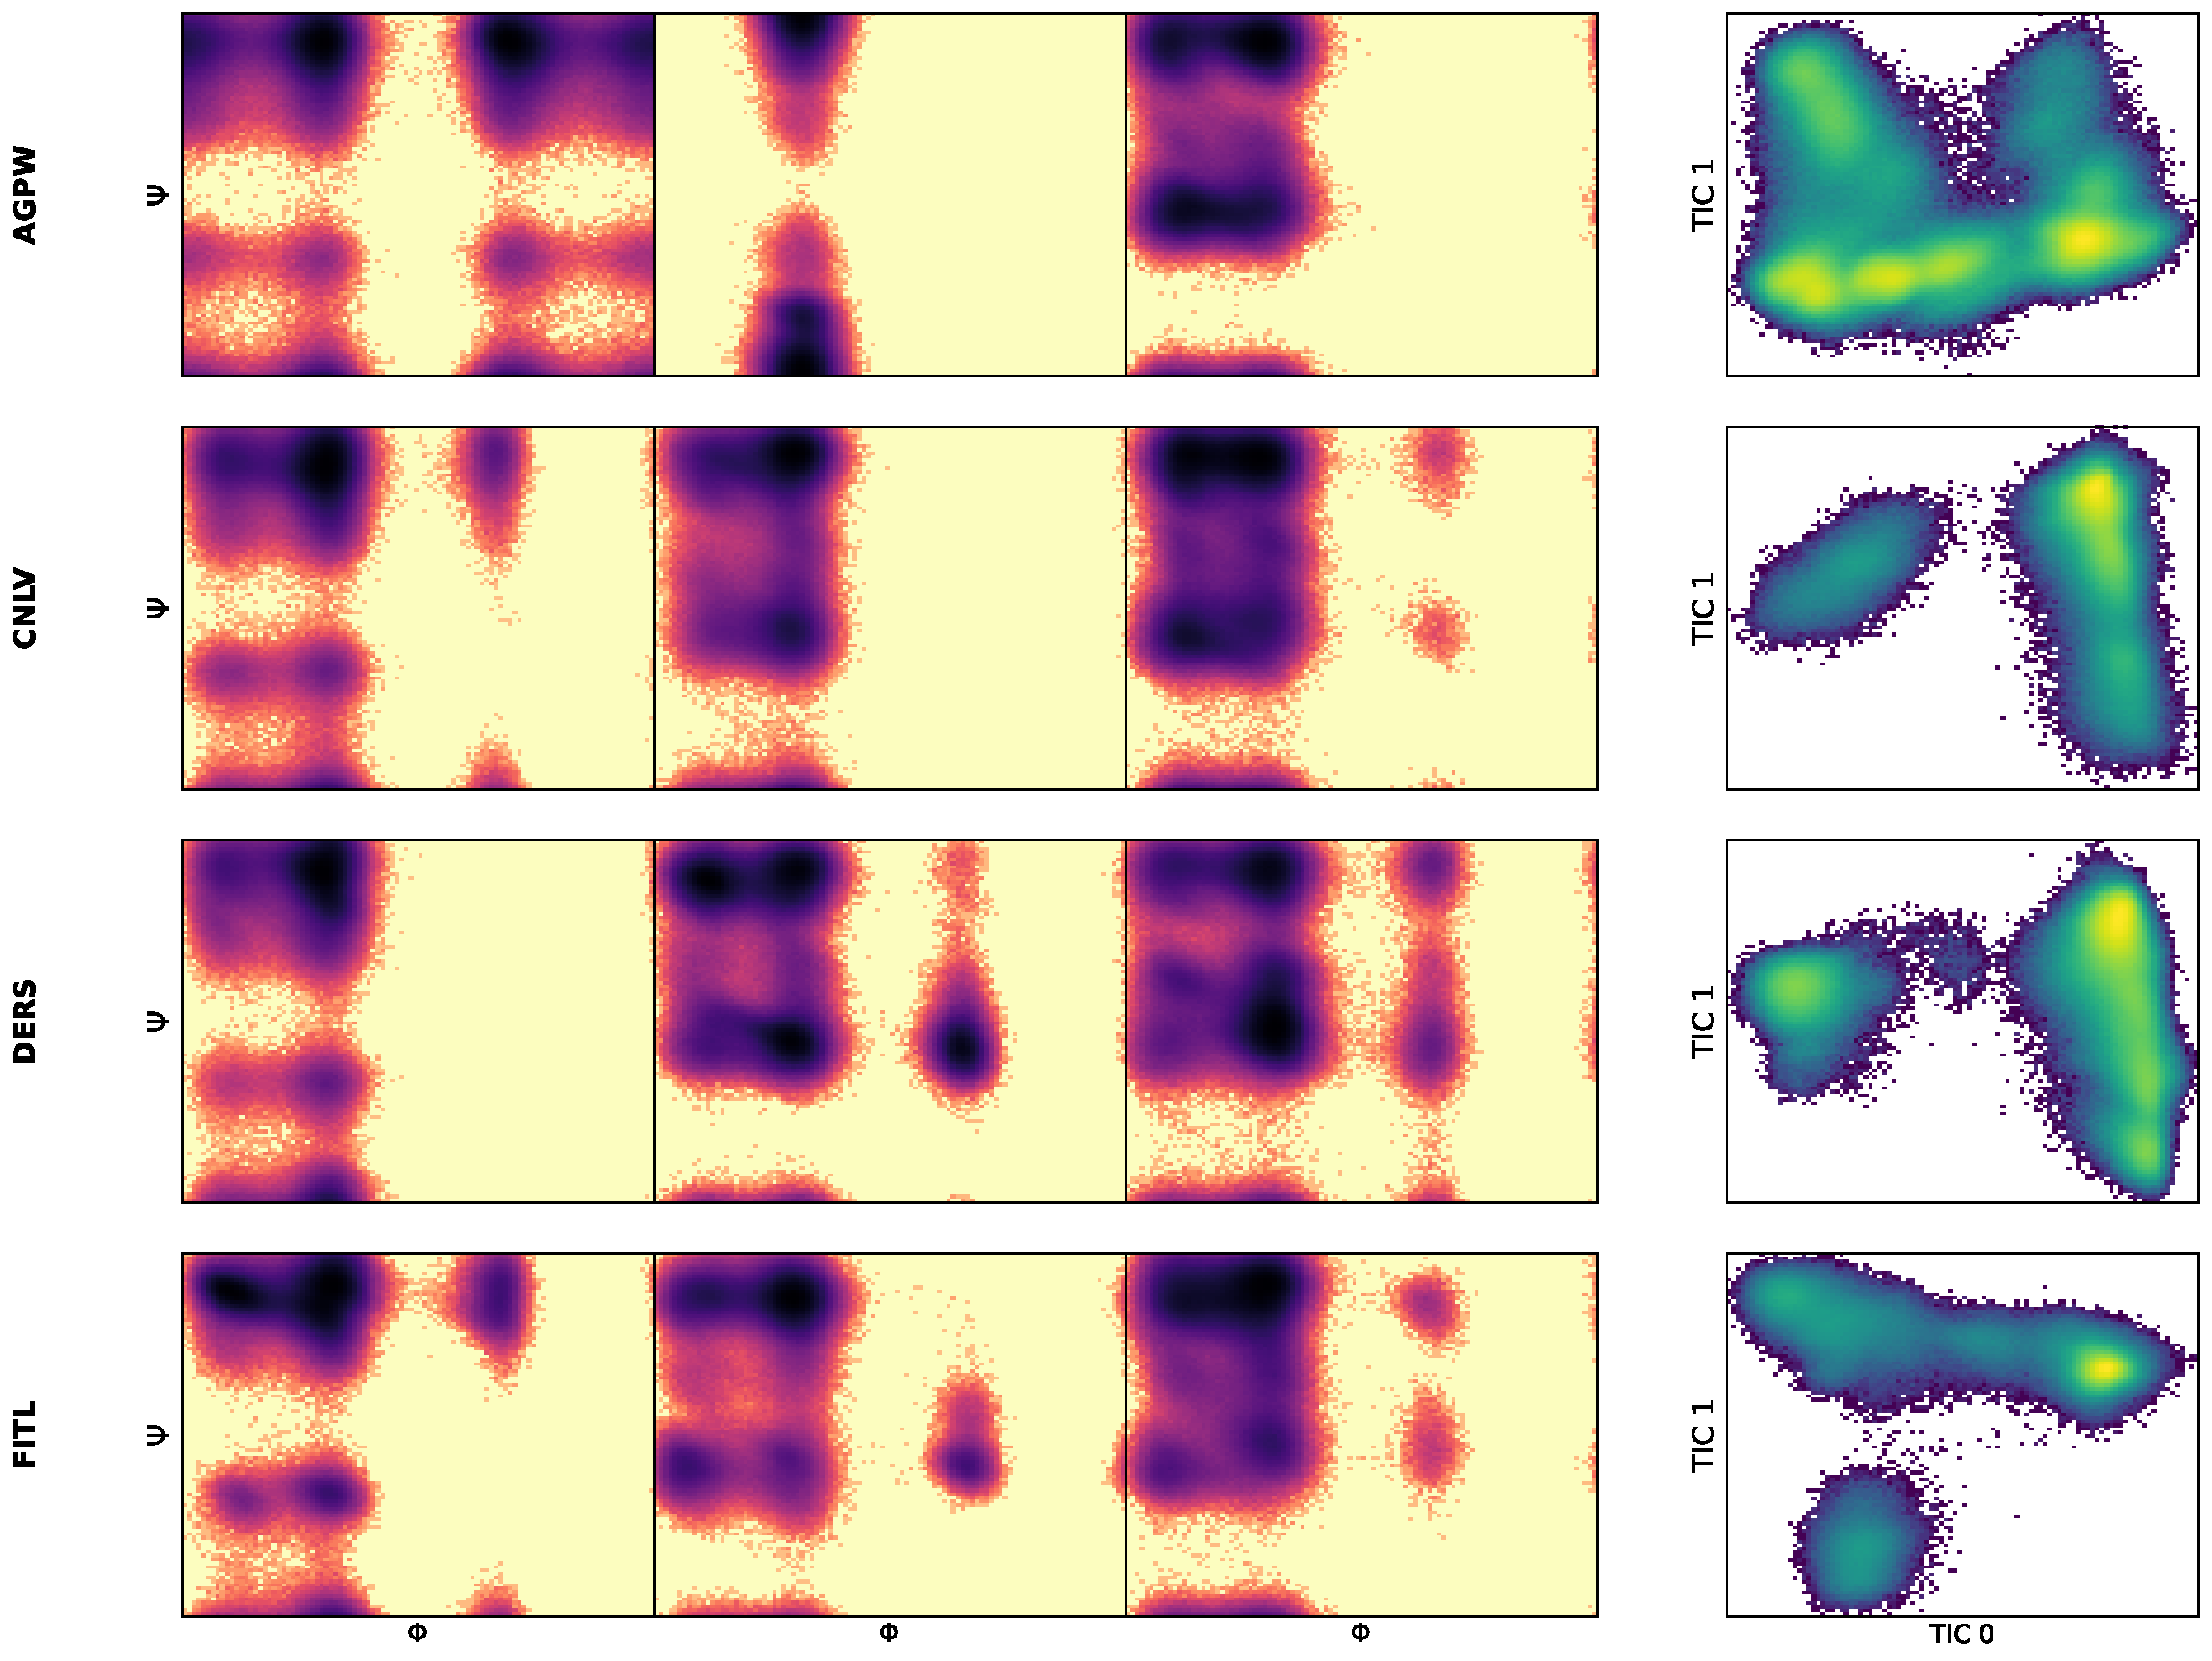
\includegraphics[width=\linewidth]{images/custom_grid_tetrapeptides_AGPW_CNLV_DERS_FITL.pdf}
    \caption{Thermodynamic and kinetic conformational landscapes of four simulated tetrapeptides (AGPW, CNLV, DERS, FITL). Each row corresponds to one tetrapeptide. \textbf{Columns 1--3:} Inter-residue Ramachandran PMFs for residue pairs 1--2, 2--3, and 3--4, characterizing local backbone torsional free-energy basins. \textbf{Column 4:} \gls{tica} projection onto TIC 0 and TIC 1, summarizing the dominant slow collective dynamics.}

    \label{fig:tetrapeptide_kinetics_thermo}
\end{figure*}

